
%(BEGIN_QUESTION)
% Copyright 2015, Tony R. Kuphaldt, released under the Creative Commons Attribution License (v 1.0)
% This means you may do almost anything with this work of mine, so long as you give me proper credit

\noindent

\vskip 5pt

\begin{center}
\textbf{Feilsøing -- Nivå 2 }
\vskip 5pt 
\textbf{Arbidsoppdrag på Stasjon 5}
\vskip 5pt 
\textbf{Feilsøing II}
\end{center}


\textbf{Introdusjon}

\vskip 5pt 

\vskip 5pt 

%$$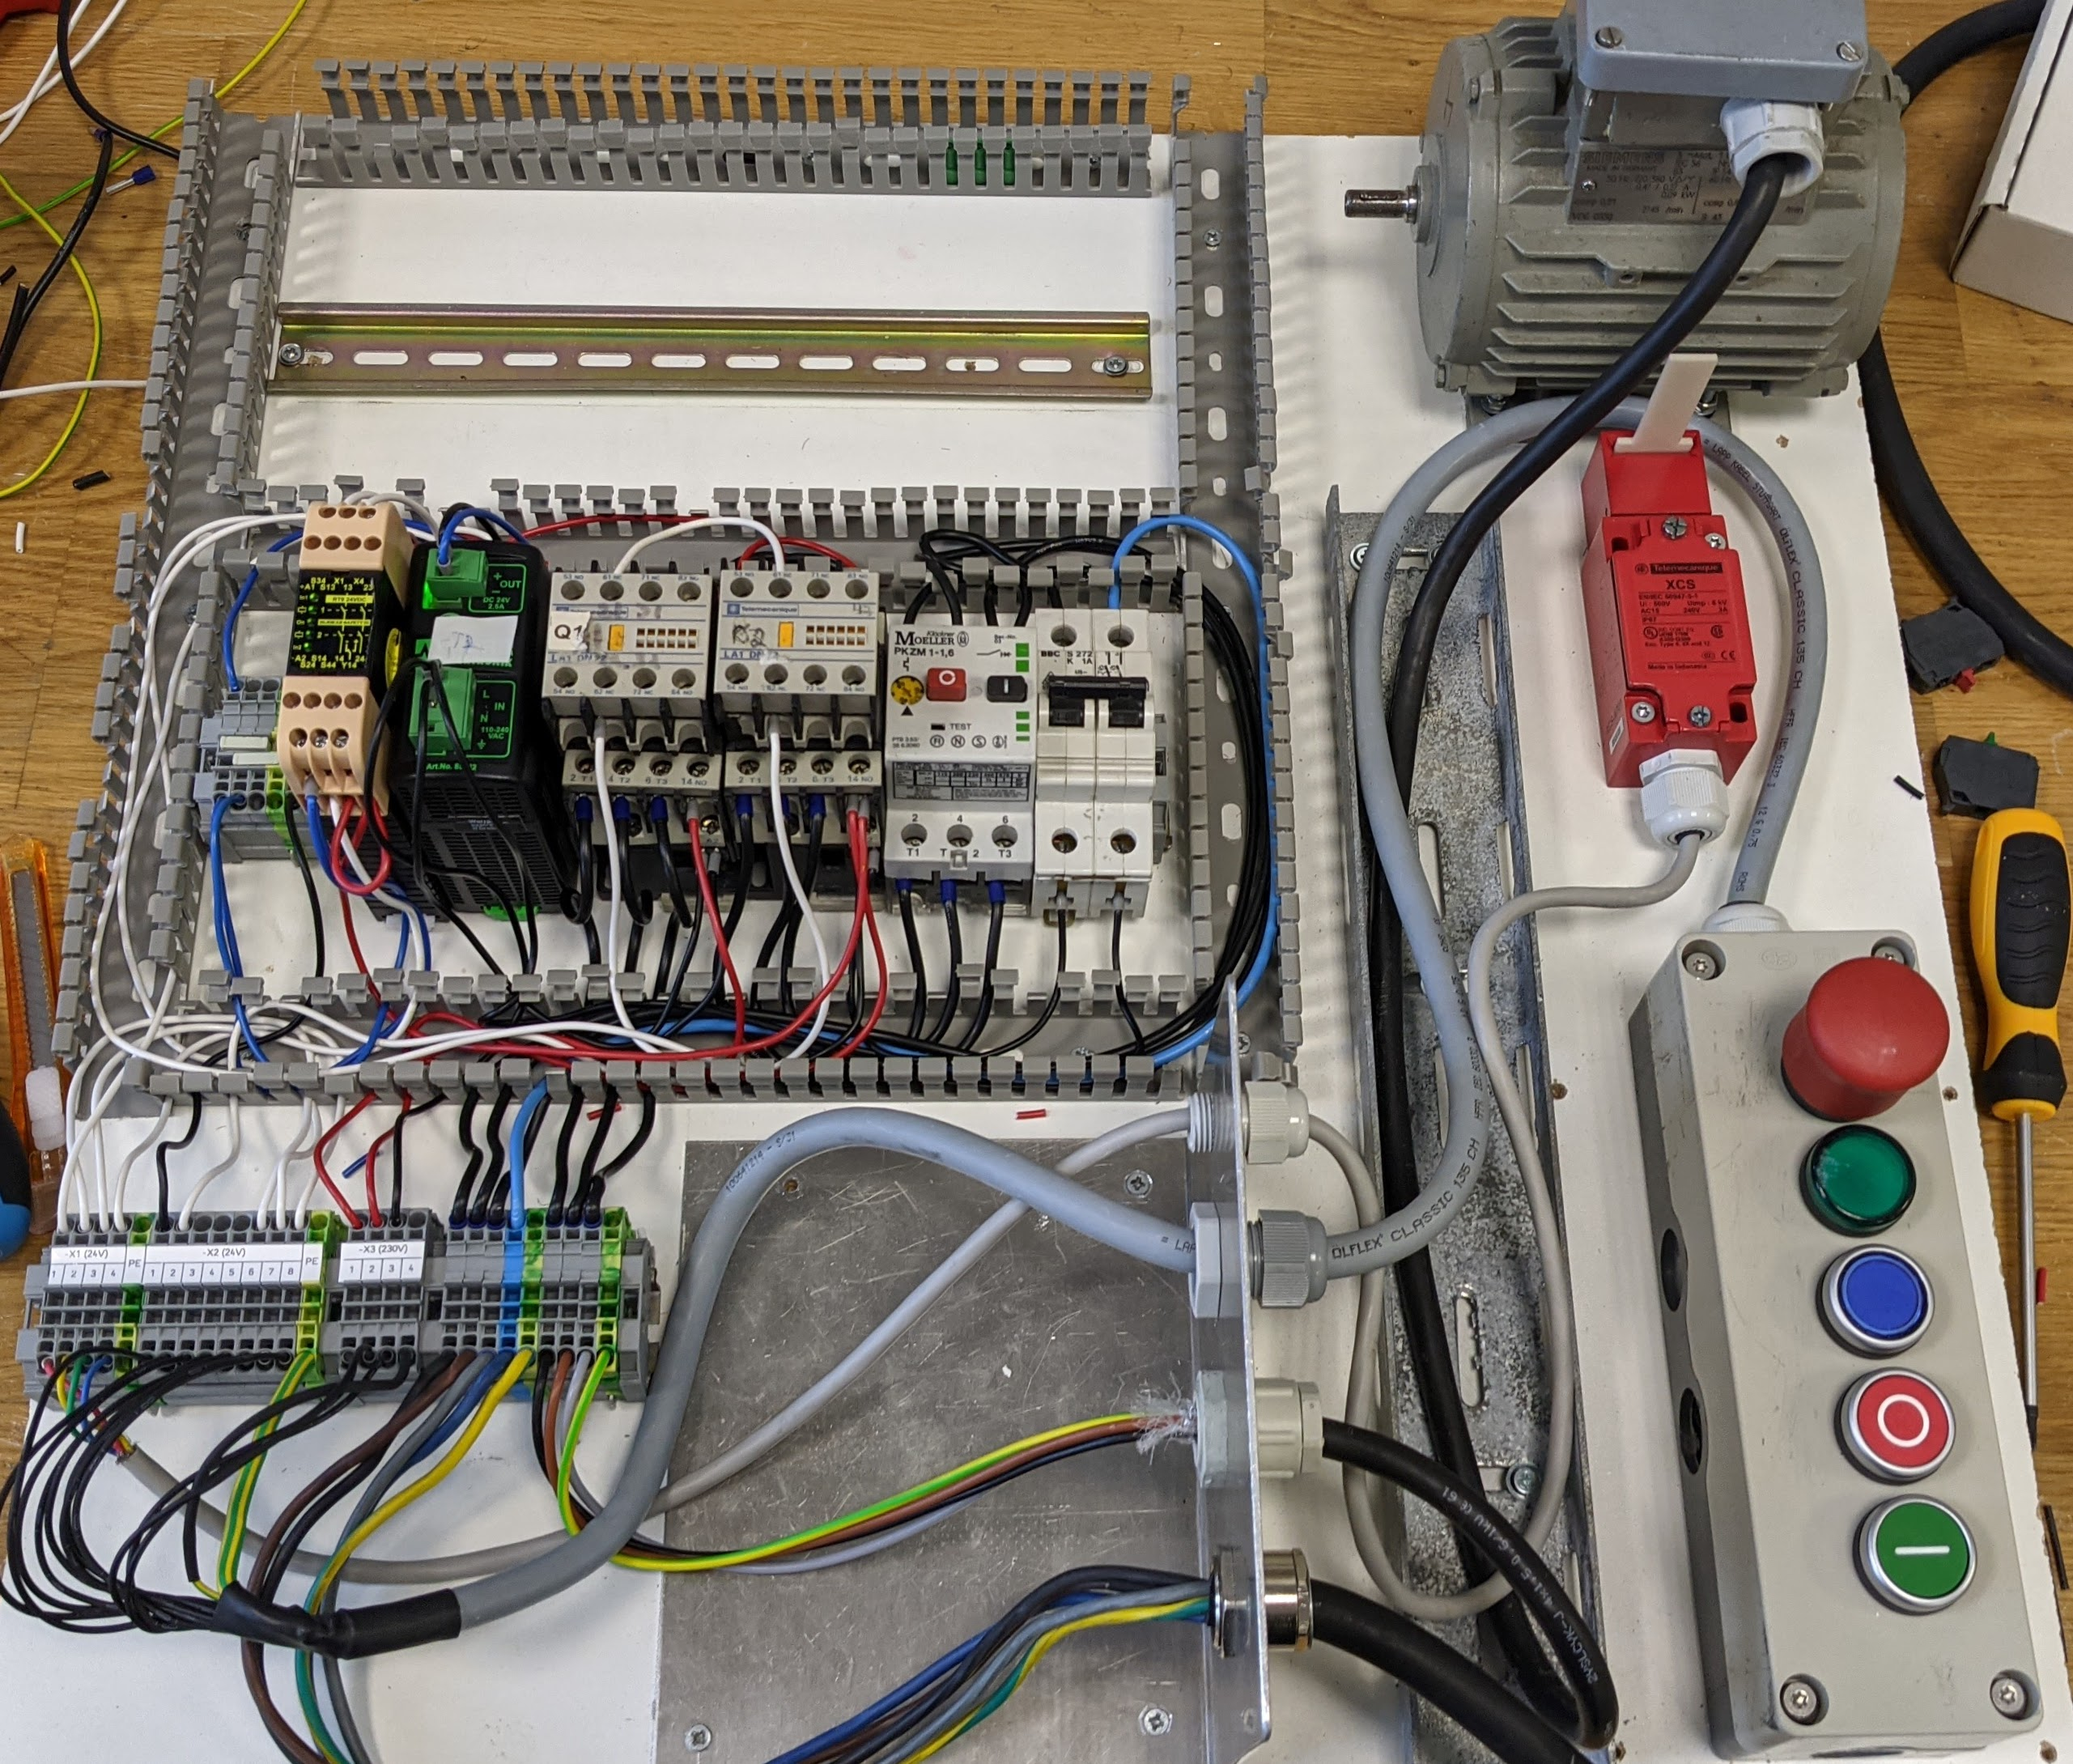
\includegraphics[width=13cm]{i04821x01.jpg}$$\\

\vskip 10pt 
\textbf{Teorioppgaver}

Start opp PLS programmet og sett deg inn i virkemåten.\\
\href{https://rfka-my.sharepoint.com/:u:/g/personal/fred-olav_mosdal_skole_rogfk_no/Ebw4MugqIk9IkNW0xOTeOtMBU5aTkfC_XWkhlCSTiTU62A?e=qM1QLI}{PLS program til stasjonen}

\vskip 5pt 
Skjema for anlegget finner du \href{https://rfka-my.sharepoint.com/:u:/g/personal/fred-olav_mosdal_skole_rogfk_no/EfUrPOgJexZLiXL5tWK_tVIBmfgED9RbsoItP9EguvaPCg?e=f5Ydh4}{her.}
\vskip 5pt 

\vskip 10pt 
\textbf{Planlegging}


\vskip 10pt 
\textbf{Gjennomføring}

\vskip 10pt 
\textbf{Dokumentasjon}

Beskriv hvordan du planlegger, gjennomfører og dokumenterer denne jobben. 





















\underbar{file i04866}
\vfil \eject
%(END_QUESTION)





%(BEGIN_ANSWER)


%(END_ANSWER)





%(BEGIN_NOTES)


%INDEX% Arbeisdoppdrag, Kompetanse, Nivå 1, Stasjonxx, Mal

%(END_NOTES)


